%==========================================================================
% report.tex -- engineering report on the serial system bus
%
% Build:  cd Serial_System_Bus/docs && latexmk -pdf report.tex
%    or:  pdflatex report.tex   (twice, for the table of contents)
%==========================================================================
\documentclass[11pt,a4paper]{article}

\usepackage[T1]{fontenc}
\usepackage[utf8]{inputenc}
\usepackage{newtxtext,newtxmath}
\usepackage[scaled=0.95]{inconsolata}
\usepackage{microtype}
\usepackage[a4paper,margin=27mm,headheight=14pt]{geometry}
\usepackage{booktabs}
\usepackage{tabularx}
\usepackage{xcolor}
\usepackage{tikz}
\usepackage{listings}
\usepackage{caption}
\usepackage{enumitem}
\usepackage{fancyhdr}
\usepackage{titlesec}
\usepackage[hidelinks]{hyperref}

\usetikzlibrary{positioning,arrows.meta,calc,decorations.pathreplacing}

%--------------------------------------------------------------------------
% Palette.  Teal for structure; clay is reserved for the superseded parallel
% design so every before/after comparison reads at a glance.
%--------------------------------------------------------------------------
\definecolor{signal}{HTML}{0B6E62}
\definecolor{legacy}{HTML}{9C5A3C}
\definecolor{rule}  {HTML}{C9D4D1}
\definecolor{muted} {HTML}{5C6B68}
\definecolor{wash}  {HTML}{EDF3F1}

\titleformat{\section}{\normalfont\large\bfseries\color{signal}}{\thesection}{0.7em}{}
\titleformat{\subsection}{\normalfont\normalsize\bfseries}{\thesubsection}{0.6em}{}
\captionsetup{font=small,labelfont={bf,color=signal}}

\pagestyle{fancy}
\fancyhf{}
\lhead{\small\color{muted}Serial System Bus}
\rhead{\small\color{muted}\thepage}
\renewcommand{\headrulewidth}{0.4pt}

\lstdefinestyle{v}{
  basicstyle=\ttfamily\footnotesize,
  keywordstyle=\color{signal}\bfseries,
  commentstyle=\color{muted},
  showstringspaces=false,
  breaklines=true,
  frame=leftline,
  framerule=1.2pt,
  rulecolor=\color{rule},
  xleftmargin=10pt,
  framexleftmargin=8pt,
  aboveskip=10pt, belowskip=8pt,
  morekeywords={module,endmodule,input,output,wire,reg,assign,always,posedge,
    negedge,begin,end,if,else,parameter,localparam,generate,endgenerate,case,
    endcase,default,integer,genvar,for}
}
\lstset{style=v}

\newcommand{\sig}[1]{\texttt{#1}}

%==========================================================================
\begin{document}

\begin{titlepage}
\centering
\vspace*{3.2cm}
{\color{signal}\rule{\textwidth}{1.2pt}}\\[4mm]
{\Huge\bfseries Design of a Serial Shared System Bus\par}
\vspace{3mm}
{\large Two masters, three slaves, priority arbitration and split
transactions on a Cyclone IV E\par}
\vspace{2mm}
{\color{signal}\rule{\textwidth}{1.2pt}}\\[10mm]

{\large rajinthanr\par}
\vspace{2mm}
{\color{muted} Digital Design --- Final Year Project Report\par}
\vspace{12mm}

\begin{minipage}{0.82\textwidth}
\small\color{muted}
\begin{tabularx}{\textwidth}{@{}lX@{}}
Target device & Altera Cyclone IV E \sig{EP4CE115F29C7} (Terasic DE2-115)\\
Synthesis     & Quartus Prime Lite 24.1std\\
Simulation    & Icarus Verilog (regression), ModelSim/Questa (waveforms)\\
Language      & Verilog-2001\\
Status        & 11 self-checking testbenches passing; timing closed at
                141.8\,MHz\\
\end{tabularx}
\end{minipage}

\vfill
{\color{muted}\small This report concerns the \emph{interconnect}. Masters and
memory slaves appear only where they define the bus contract.\par}
\vspace{8mm}
\end{titlepage}

\tableofcontents
\newpage

%==========================================================================
\section{Scope and summary}

This report covers the design of the \textbf{bus} --- arbitration, address
decoding, the shared signalling wires, the transfer protocol, the split
mechanism, and the guarantee that the bus cannot hang. The masters and the
memory slaves are treated as endpoints: they appear where they define or
constrain the bus contract, and not otherwise.

The headline result is a shared bus in which \textbf{the address and the data
each travel on a single wire}. The shared segment is eight wires, down from
eighty-six in the parallel design it replaced, and the total net count across
the interconnect falls from 337 to 60. The cost is time: a write takes 21
clocks instead of 5, a read 30 instead of 5. The design still closes timing
at 141.8\,MHz against a 50\,MHz requirement, and is slightly \emph{smaller}
than the parallel bus it replaced.

\begin{table}[htb]
\centering\small
\caption{Summary of the two architectures. All figures measured, not estimated.}
\begin{tabular}{@{}lrr@{}}
\toprule
& \textcolor{legacy}{\textbf{Parallel}} & \textcolor{signal}{\textbf{Serial}}\\
\midrule
Shared bus wires        & 86         & \textbf{8}\\
Total interconnect nets & 337        & \textbf{60}\\
Write latency           & 5\,clk     & 21\,clk\\
Read latency            & 5\,clk     & 30\,clk\\
Split read latency      & 16\,clk    & 79\,clk\\
Logic elements          & 721        & \textbf{688}\\
Registers               & 544        & \textbf{513}\\
$F_{\max}$              & 117.7\,MHz & \textbf{141.8\,MHz}\\
\bottomrule
\end{tabular}
\end{table}

%==========================================================================
\section{Requirements and constraints}

The bus had to support two masters and three memory slaves of 4\,KB, 4\,KB
and 2\,KB, with priority arbitration, address decoding, and AHB-style split
transactions. Four constraints shaped every decision that follows.

\begin{description}[leftmargin=1.4em,style=nextline,font=\bfseries]
\item[One clock domain, one asynchronous reset.]
No gated clocks, no derived clocks, no second domain anywhere in the
interconnect. This later ruled out the obvious way of slowing the board demo
down (\S\ref{sec:limits}).

\item[The bus must never hang.]
An access to an unmapped address had to complete, not stall. This is a
property of the bus, and it drove a specific structural decision
(\S\ref{sec:hang}).

\item[Parameterised for three requesters.]
A later phase adds a bridge to a second board as a third bus master, so the
arbiter could not be hard-coded for two.

\item[The split mechanism written once.]
The same phase reuses it for the remote bridge, which will be slow for
exactly the same reason a busy slave is.
\end{description}

A 16-bit word address was fixed by the address map: three slaves at
\sig{0x0000}, \sig{0x1000} and \sig{0x2000}, with \sig{addr[15]} reserved for
the future remote window and deliberately left unmapped.

%==========================================================================
\section{Decisions taken before writing RTL}

The specification left several bus-level questions open. Fixing them first,
in writing, was worth the half hour it took: each one is a contract that
several modules must agree on, and discovering a disagreement in simulation
is far more expensive than deciding it up front.

\begin{table}[htb]
\centering\small
\caption{Bus-level decisions and their reasoning.}
\begin{tabularx}{\textwidth}{@{}llX@{}}
\toprule
\textbf{Question} & \textbf{Decision} & \textbf{Reasoning}\\
\midrule
Response encoding & \sig{OKAY}=00, \sig{ERROR}=01, \sig{SPLIT}=10 &
AHB-flavoured. \sig{OKAY} is all-zero, so a reset or an idle bus reads as
``nothing wrong''.\\
\addlinespace
Handshake polarity & active high, except \sig{rst\_n} &
One rule, with no exceptions to remember.\\
\addlinespace
Data width & 8 bits &
On a serial bus this is a direct latency cost --- one clock per bit on every
transfer. It also makes the slaves 4\,KB/4\,KB/2\,KB, the natural reading of
the sizes given.\\
\addlinespace
Retry policy on \sig{ERROR} & report, never retry &
An unmapped address will not become mapped. A retry is an infinite loop
holding the bus.\\
\addlinespace
Split visibility & invisible to the requester &
One command in, one completion out, however many times the transfer was
actually driven. The replay is the bus's business.\\
\bottomrule
\end{tabularx}
\end{table}

%==========================================================================
\section{First architecture: a parallel multiplexed bus}
\label{sec:parallel}

The first implementation was a conventional parallel bus. It is worth
recording, because it establishes the baseline the serial design is measured
against, and because building it surfaced one fact that governs everything
afterwards.

\subsection{A ``shared bus'' on an FPGA is a multiplexer}

The textbook shared bus is wired-OR or tri-stated: every master drives the
same physical conductor and only one enables its driver at a time.
\textbf{An FPGA has no internal tri-state buffers.} Quartus will accept an
\sig{inout} on an internal net and then silently convert it into exactly the
multiplexer one would have written by hand, so there is nothing to be gained
by pretending otherwise.

The design therefore has no \sig{inout} ports and no \sig{z} values anywhere.
``Sharing'' means:

\begin{itemize}[leftmargin=1.4em,itemsep=1pt]
\item a \emph{forward} multiplexer selected by the arbiter's one-hot grant,
      putting the granted master's signals onto the bus;
\item a \emph{return} multiplexer selected by a copy of the decoder's select,
      putting the responding slave's reply back.
\end{itemize}

Each master has its own private bundle of wires running to the multiplexer;
the shared segment exists only downstream of it.

\subsection{The wire census}

Counting nets made the cost of the parallel approach concrete.

\begin{table}[htb]
\centering\small
\caption{Parallel bus net count. The shared segment is what every endpoint taps.}
\begin{tabular}{@{}lrrr@{}}
\toprule
\textbf{Segment} & \textbf{Per unit} & \textbf{Units} & \textbf{Nets}\\
\midrule
Master $\rightarrow$ forward mux (private) & 50 & 2 & 100\\
Shared forward (mux $\rightarrow$ slaves)  & 51 & 1 & 51\\
Slave $\rightarrow$ return mux (private)   & 35 & 4 & 140\\
Shared return (broadcast to masters)       & 35 & 1 & 35\\
Arbitration and select                     & 11 & 1 & 11\\
\midrule
\multicolumn{3}{@{}l}{\textbf{Total}} & \textbf{337}\\
\multicolumn{3}{@{}l}{\emph{of which shared}} & \emph{86}\\
\bottomrule
\end{tabular}
\end{table}

The parallel bus worked and passed a full test suite at five clocks per
transfer. But eighty-six wires between every endpoint is precisely the cost a
serial bus exists to avoid, and the project called for a serial one.

%==========================================================================
\section{Re-specification: serial signalling}

The requirement is simple to state and expensive to satisfy: \textbf{the
address travels on one wire and the data on one wire}, shared by every master
and every slave.

Three consequences follow immediately, and each is a design problem rather
than a coding detail.

\begin{enumerate}[leftmargin=1.6em,itemsep=2pt]
\item \textbf{A 16-bit address costs 16 clocks}, on every transfer,
      unavoidably. Latency stops being a rounding error and becomes the
      dominant characteristic of the bus.

\item \textbf{The decoder cannot decide anything until the frame ends.}
      In the parallel design the address was present in one cycle and the
      select followed combinationally. Here no slave knows whether it is the
      target until the last address bit has landed.

\item \textbf{The reply is no longer at a fixed offset from the address.}
      A write can be answered immediately; a read cannot answer until it has
      shifted its data out. Anything that assumed a fixed reply time ---
      and the parallel return path did --- breaks.
\end{enumerate}

The interesting engineering is in points 2 and 3. Point 1 is simply the price.

%==========================================================================
\section{The serial bus}

\subsection{Eight wires}

\begin{table}[htb]
\centering\small
\caption{The complete shared bus. Everything else is point-to-point.}
\begin{tabularx}{\textwidth}{@{}llX@{}}
\toprule
\textbf{Wire} & \textbf{Width} & \textbf{Role}\\
\midrule
\sig{bus\_astream} & 1 & The address. Driven by the granted master; received
                         by every slave and by the decoder's deserialiser.\\
\sig{bus\_dstream} & 1 & The data. Half duplex.\\
\sig{bus\_valid}   & 1 & Frame marker, high for \sig{ADDR\_W} clocks.\\
\sig{bus\_we}      & 1 & Direction; also the data wire's direction control.\\
\sig{bus\_ready}   & 1 & Completion strobe.\\
\sig{bus\_resp}    & 2 & \sig{OKAY} / \sig{ERROR} / \sig{SPLIT}.\\
\sig{master\_id}   & 1 & Tag of the granted master, so a split-capable slave
                         can record whose transfer it deferred.\\
\bottomrule
\end{tabularx}
\end{table}

\begin{figure}[htb]
\centering
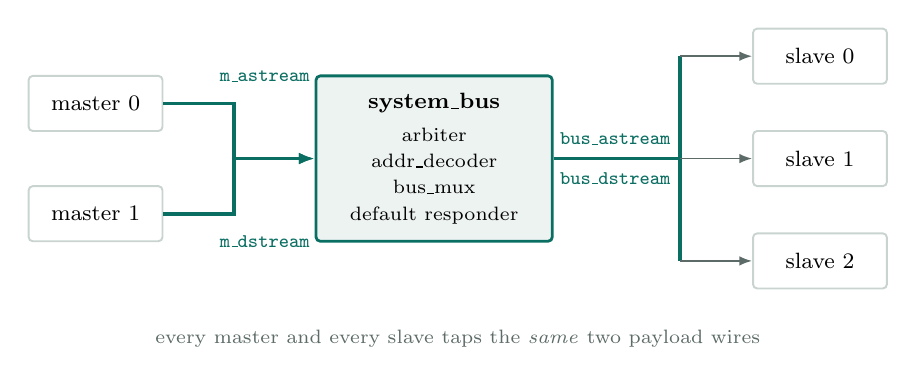
\begin{tikzpicture}[
  font=\footnotesize,
  box/.style={draw=rule,line width=0.7pt,rounded corners=1.5pt,fill=white,
              minimum height=7mm,minimum width=17mm,align=center},
  bus/.style={draw=signal,line width=1.4pt},
  lbl/.style={font=\scriptsize\ttfamily,color=signal},
  tap/.style={draw=muted,line width=0.6pt}]

\node[box] (m0) at (0,1.7) {master 0};
\node[box] (m1) at (0,0.3) {master 1};

\node[box,minimum width=30mm,minimum height=21mm,fill=wash,draw=signal,
      line width=1pt] (bus) at (4.3,1.0)
  {\textbf{system\_bus}\\[0.8mm]
   \scriptsize arbiter\\\scriptsize addr\_decoder\\\scriptsize bus\_mux\\
   \scriptsize default responder};

\node[box] (s0) at (9.2,2.3) {slave 0};
\node[box] (s1) at (9.2,1.0) {slave 1};
\node[box] (s2) at (9.2,-0.3) {slave 2};

\draw[bus,-{Latex[length=2mm]}] (m0.east) -- ++(0.9,0) |- (bus.west);
\draw[bus,-{Latex[length=2mm]}] (m1.east) -- ++(0.9,0) |- (bus.west);
\node[lbl,anchor=south] at (2.15,1.85) {m\_astream};
\node[lbl,anchor=north] at (2.15,0.15) {m\_dstream};

\draw[bus] (bus.east) -- ++(1.6,0) coordinate (spine);
\node[lbl,anchor=south] at (6.6,1.05) {bus\_astream};
\node[lbl,anchor=north] at (6.6,0.95) {bus\_dstream};
\draw[bus] ($(spine)+(0,-1.3)$) -- ($(spine)+(0,1.3)$);
\draw[tap,-{Latex[length=1.6mm]}] ($(spine)+(0,1.3)$) -- (s0.west);
\draw[tap,-{Latex[length=1.6mm]}] (spine) -- (s1.west);
\draw[tap,-{Latex[length=1.6mm]}] ($(spine)+(0,-1.3)$) -- (s2.west);

\node[color=muted,font=\scriptsize,anchor=north] at (4.6,-1.05)
  {every master and every slave taps the \emph{same} two payload wires};
\end{tikzpicture}
\caption{Bus topology. The shared segment is two payload wires plus six
control wires; every per-endpoint stub is one bit.}
\end{figure}

\subsection{The frame, and the one choice that made it cheap}
\label{sec:frame}

An address phase is \sig{ADDR\_W}${=}16$ clocks with \sig{bus\_valid} high.
The address goes out most-significant bit first. On a write, the data goes
out on the other wire \emph{at the same time} --- and \textbf{right-aligned}.

\begin{figure}[htb]
\centering
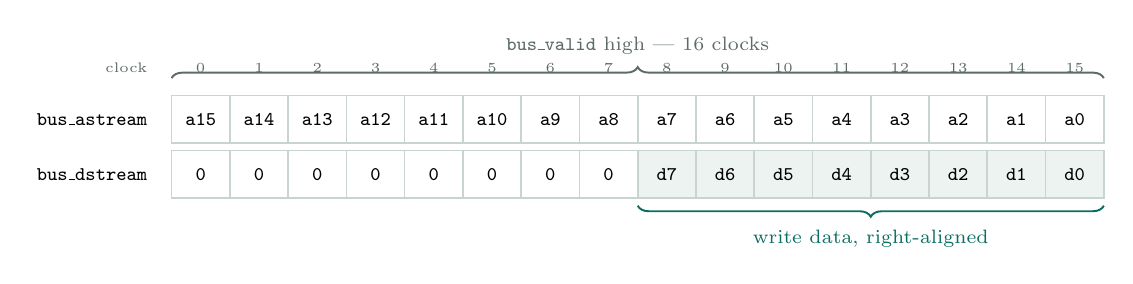
\begin{tikzpicture}[font=\scriptsize,x=7.4mm,y=1cm]
  \def\slot#1#2#3#4{%
    \draw[draw=rule,line width=0.6pt,fill=#4] (#1,#2) rectangle ++(1,0.6);
    \node[font=\scriptsize\ttfamily] at (#1+0.5,#2+0.3) {#3};}

  \foreach \i in {0,...,15}{\node[color=muted,font=\tiny] at (\i+0.5,2.15) {\i};}
  \node[color=muted,font=\tiny,anchor=east] at (-0.25,2.15) {clock};

  \node[anchor=east,font=\scriptsize\ttfamily] at (-0.25,1.5) {bus\_astream};
  \foreach \i/\b in {0/a15,1/a14,2/a13,3/a12,4/a11,5/a10,6/a9,7/a8,
                     8/a7,9/a6,10/a5,11/a4,12/a3,13/a2,14/a1,15/a0}{
    \slot{\i}{1.2}{\b}{white}}

  \node[anchor=east,font=\scriptsize\ttfamily] at (-0.25,0.8) {bus\_dstream};
  \foreach \i in {0,...,7}{\slot{\i}{0.5}{0}{white}}
  \foreach \i/\b in {8/d7,9/d6,10/d5,11/d4,12/d3,13/d2,14/d1,15/d0}{
    \slot{\i}{0.5}{\b}{wash}}

  \draw[decorate,decoration={brace,amplitude=4pt,mirror},color=signal,
        line width=0.7pt] (8,0.4) -- (16,0.4)
    node[midway,below=5pt,color=signal,font=\scriptsize]
    {write data, right-aligned};
  \draw[decorate,decoration={brace,amplitude=4pt},color=muted,
        line width=0.7pt] (0,2.02) -- (16,2.02)
    node[midway,above=5pt,color=muted,font=\scriptsize]
    {\texttt{bus\_valid} high --- 16 clocks};
\end{tikzpicture}
\caption{The address frame. Padding the write data with leading zeros costs
nothing and removes every bit counter from the receiving side.}
\label{fig:frame}
\end{figure}

Right-aligning the data is the single most useful decision in the design.
Because the data sits at the \emph{end} of the frame, every receiver can be a
plain shift register of its own width, clocked for the whole frame, holding
\emph{the last $W$ bits it saw} --- and that is exactly the field it wanted.

\begin{table}[htb]
\centering\small
\caption{Four receivers, one wire, no bit counters.}
\begin{tabular}{@{}llll@{}}
\toprule
\textbf{Receiver} & \textbf{Width} & \textbf{Ends up holding} & \textbf{Discards}\\
\midrule
Central deserialiser (for the decoder) & 16 & the whole address & ---\\
Slave 0 / slave 1 address & 12 & \sig{addr[11:0]}, its offset & \sig{addr[15:12]}\\
Slave 2 address           & 11 & \sig{addr[10:0]}, its offset & \sig{addr[15:11]}\\
Any slave's write data    & 8  & the data byte & the padding\\
\bottomrule
\end{tabular}
\end{table}

The upper address bits shift straight through a slave's narrow register and
fall off the end; deciding \emph{which} slave is the decoder's job, and it is
the only receiver that needs all sixteen bits. The result is that
\textbf{there is exactly one frame timer on the entire bus} --- a counter
inside the granted master --- and every other endpoint simply follows
\sig{bus\_valid}. The serialiser makes the padding automatic by shifting
zeros in behind the data:

\begin{lstlisting}
always @(posedge clk or negedge rst_n) begin
    if (!rst_n)     sr <= {W{1'b0}};
    else if (load)  sr <= din;
    else if (shift) sr <= {sr[W-2:0], 1'b0};   // zeros in behind
end
assign dout = sr[W-1];
\end{lstlisting}

\subsection{Decode has to happen after the frame}

Since no slave knows whether it is selected until the last address bit
arrives, \textbf{every slave shifts every frame in, addressed or not}, and
selection arrives afterwards as a one-cycle pulse. Shifting speculatively
costs nothing: a slave that was not selected never acts on what it collected.
The corresponding hazard --- a slave acting on a frame without a select, and
corrupting another slave's transfer --- is tested directly
(\S\ref{sec:verif}).

The decode strobe is derived rather than transmitted:

\begin{lstlisting}
reg bus_valid_d;
always @(posedge clk or negedge rst_n)
    if (!rst_n) bus_valid_d <= 1'b0;
    else        bus_valid_d <= bus_valid;

assign addr_done = bus_valid_d & ~bus_valid;   // falling edge of the frame
\end{lstlisting}

Using the falling edge of \sig{bus\_valid} rather than adding an
``end of frame'' wire keeps the shared bus at eight wires and --- more
usefully --- leaves the frame length defined in exactly one place. Nothing
else on the bus knows or cares how long a frame is.

A pleasant consequence: the address decoder is \textbf{unchanged} from the
parallel design. It is still purely combinational, address in and one-hot
select out; it is simply enabled for one cycle per frame instead of one cycle
per access.

\subsection{The data wire needs no turnaround}

A half-duplex wire normally needs a turnaround cycle and some way to stop two
drivers overlapping. This one does not, because the two directions cannot
overlap by construction:

\begin{center}\small
\begin{tabular}{@{}lll@{}}
\toprule
& \textbf{During the frame} & \textbf{After the frame}\\
\midrule
Write & master sends & ---\\
Read  & ---          & slave sends\\
\bottomrule
\end{tabular}
\end{center}

So the direction control is nothing more than \sig{bus\_we}, which the
granted master holds stable for the whole transaction:

\begin{lstlisting}
assign bus_dstream = bus_we ? m_dstream_sel : s_dstream_sel;
\end{lstlisting}

The master explicitly releases the wire on a read, and each slave drives only
while actually shifting data out. Both are belt-and-braces given the
multiplexer above, but they keep an idle bus readable in a waveform, and a
testbench asserts that the master never drives during a read.

\subsection{The return select had to become a latch}

This is the correction serialisation forced, and it is worth spelling out
because the parallel design's approach looks correct until it is not.

In the parallel bus a reply always came back exactly one cycle after the
address, so the return multiplexer was steered by a one-cycle-delayed copy of
the decoder select --- a single register.

On the serial bus the reply offset is variable:

\begin{table}[htb]
\centering\small
\caption{Completion timing, measured from the select pulse $S$.}
\begin{tabular}{@{}lll@{}}
\toprule
\textbf{Case} & \textbf{Ready at} & \textbf{Why}\\
\midrule
Write       & $S{+}1$  & the word is committed at $S$\\
\sig{SPLIT} & $S{+}1$  & the slave is getting out of the way\\
Unmapped    & $S{+}1$  & the default responder answers at once\\
Read        & $S{+}10$ & memory access, then eight bits shifted out\\
\bottomrule
\end{tabular}
\end{table}

A one-cycle-delayed select goes stale nine cycles before a read reply
arrives. The select is therefore \emph{captured} on the decoder's pulse and
\emph{held} until the next transfer selects something else. That is safe
precisely because the arbiter locks the bus: only one transfer is ever
outstanding.

\begin{lstlisting}
always @(posedge clk or negedge rst_n) begin
    if (!rst_n)    sel_q <= {(N_SLAVES+1){1'b0}};
    else if (|sel) sel_q <= sel;        // capture and HOLD
end
\end{lstlisting}

\begin{figure}[htb]
\centering
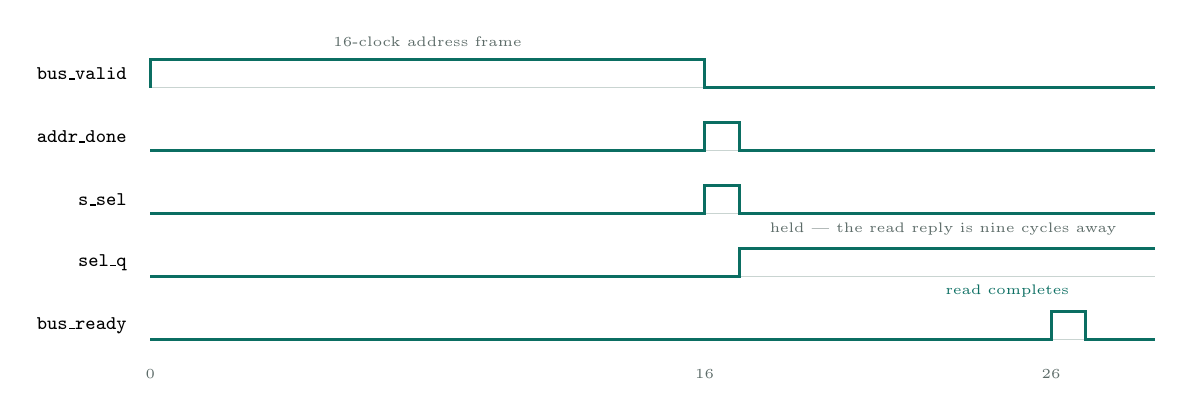
\begin{tikzpicture}[font=\scriptsize,x=4.4mm,y=1cm]
  \foreach \name/\y in {{bus\_valid}/3.2,{addr\_done}/2.4,{s\_sel}/1.6,
                        {sel\_q}/0.8,{bus\_ready}/0.0}{
    \node[anchor=east,font=\scriptsize\ttfamily] at (-0.4,\y+0.18) {\name};
    \draw[color=rule,line width=0.5pt] (0,\y) -- (29,\y);}
  \draw[signal,line width=1.1pt] (0,3.2)--(0,3.56)--(16,3.56)--(16,3.2)--(29,3.2);
  \draw[signal,line width=1.1pt] (0,2.4)--(16,2.4)--(16,2.76)--(17,2.76)--(17,2.4)--(29,2.4);
  \draw[signal,line width=1.1pt] (0,1.6)--(16,1.6)--(16,1.96)--(17,1.96)--(17,1.6)--(29,1.6);
  \draw[signal,line width=1.1pt] (0,0.8)--(17,0.8)--(17,1.16)--(29,1.16);
  \draw[signal,line width=1.1pt] (0,0.0)--(26,0.0)--(26,0.36)--(27,0.36)--(27,0.0)--(29,0.0);
  \node[color=muted,font=\tiny,anchor=south] at (8,3.60) {16-clock address frame};
  \node[color=muted,font=\tiny,anchor=south west] at (17.6,1.20)
       {held --- the read reply is nine cycles away};
  \node[color=signal,font=\tiny,anchor=south east] at (26.8,0.42) {read completes};
  \foreach \i in {0,16,26}{\node[color=muted,font=\tiny] at (\i,-0.44) {\i};}
\end{tikzpicture}
\caption{A read. The select is a one-cycle pulse; the \emph{latched} copy is
what routes the reply nine cycles later.}
\end{figure}

%==========================================================================
\section{Arbitration}

Fixed priority, master~0 highest, with two mechanisms layered on top.

\paragraph{Bus lock.} Once a master is granted, the grant is held until that
transfer completes, so a transfer is never torn in half. The arbiter
re-arbitrates on the cycle after completion, which stops a high-priority
master owning the bus across a whole burst while keeping each transfer
atomic. This matters far more after serialisation: the lock now spans 21 to
30 clocks rather than 5, so a lock that released early would open a much
larger window of corruption.

\paragraph{Split mask.} One bit per master. A master whose transfer is
answered \sig{SPLIT} has its mask bit set and is removed from arbitration
entirely; the bit is cleared when the slave signals completion. Crucially,
\textbf{the deferred master keeps its request asserted the whole time}.
Masking, not request withdrawal, is what defers it. That keeps the decision
about \emph{when} to replay inside the master and leaves the arbiter a pure
scheduler.

\paragraph{Parameterisation.} \sig{N\_MASTERS} and \sig{ID\_W} are
parameters, the priority encoder is a loop, and the mask is a per-bit vector,
so the phase-2 bridge joins as requester~2 without touching the logic. The
arbiter is also the one module that \textbf{did not change at all} when the
bus was serialised: it only ever observed \sig{req}, \sig{bus\_ready} and
\sig{bus\_resp}, none of which are serial.

%==========================================================================
\section{Split transactions}

\begin{figure}[htb]
\centering
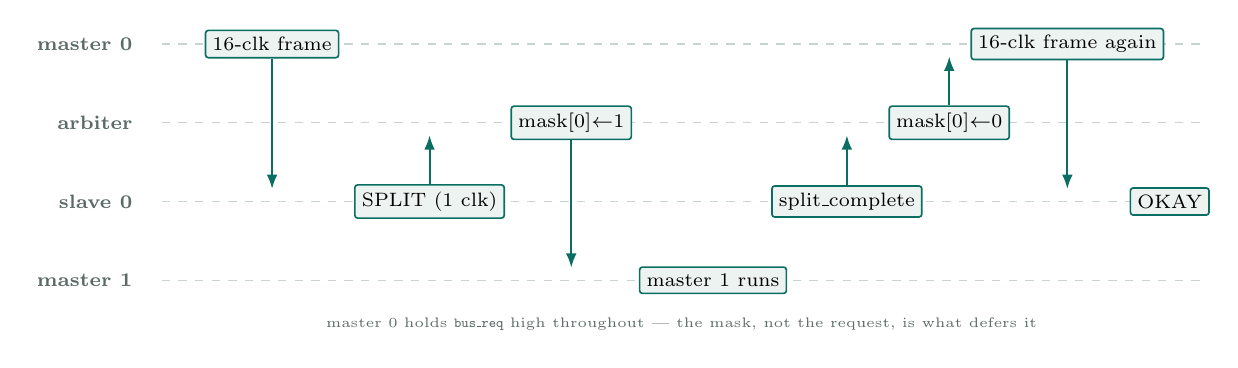
\begin{tikzpicture}[font=\scriptsize,
  lane/.style={color=muted,font=\scriptsize\bfseries},
  ev/.style={draw=signal,fill=wash,line width=0.6pt,rounded corners=1pt,
             inner sep=2.5pt,font=\scriptsize},
  ar/.style={-{Latex[length=1.8mm]},color=signal,line width=0.7pt}]
  \foreach \n/\y in {{master 0}/3.0,{arbiter}/2.0,{slave 0}/1.0,{master 1}/0.0}{
    \node[lane,anchor=east] at (-0.25,\y) {\n};
    \draw[color=rule,line width=0.5pt,dashed] (0,\y) -- (13.2,\y);}

  \node[ev] (f1) at (1.4,3.0) {16-clk frame};
  \draw[ar] (f1.south) -- (1.4,1.16);
  \node[ev] (sp) at (3.4,1.0) {SPLIT (1 clk)};
  \draw[ar] (sp.north) -- (3.4,1.84);
  \node[ev] (mk) at (5.2,2.0) {mask[0]$\leftarrow$1};
  \draw[ar] (mk.south) -- (5.2,0.16);
  \node[ev]      at (7.0,0.0) {master 1 runs};
  \node[ev] (dn) at (8.7,1.0) {split\_complete};
  \draw[ar] (dn.north) -- (8.7,1.84);
  \node[ev] (um) at (10.0,2.0) {mask[0]$\leftarrow$0};
  \draw[ar] (um.north) -- (10.0,2.84);
  \node[ev] (f2) at (11.5,3.0) {16-clk frame again};
  \draw[ar] (f2.south) -- (11.5,1.16);
  \node[ev] at (12.8,1.0) {OKAY};

  \node[color=muted,font=\tiny,anchor=north] at (6.6,-0.35)
    {master 0 holds \texttt{bus\_req} high throughout --- the mask, not the
     request, is what defers it};
\end{tikzpicture}
\caption{A split transaction. The replay re-transmits the complete frame; it
is a re-issue, not a resumption.}
\end{figure}

Three properties define the mechanism at bus level.

\begin{description}[leftmargin=1.4em,style=nextline,font=\bfseries]
\item[The deferred transfer is not performed.]
No write lands, no read happens. Since the master re-transmits the entire
frame, the slave only has to remember \emph{who} it deferred --- one master
ID --- and no address or data storage is needed anywhere in the split logic.

\item[The replay is a complete frame,]
not a resumption of a half-finished one. This is verified explicitly: a split
transaction must put \emph{two} full-length frames on the wire.

\item[One split outstanding.]
An access arriving while the slave is busy, or while a resume is still owed,
is served normally. This is a deliberate simplification: with single-entry
deferred state, allowing a second split would mask two masters with only one
wake-up available to release them --- a deadlock.
\end{description}

\paragraph{Why splitting earns its keep here.} On the parallel bus the
asymmetry was mild: a split freed the bus for a handful of clocks. On the
serial bus a slave answers \sig{SPLIT} in \textbf{one} clock while a real
read costs \textbf{ten}, and the whole transaction costs thirty. Deferring
therefore hands the other master a genuinely useful window. Serialisation did
not merely slow the bus down --- it turned a mechanism that was close to
decorative into one that does real work.

%==========================================================================
\section{The bus must not hang}
\label{sec:hang}

Without a responder for unmapped addresses, an access to a decode hole
asserts no slave select, nothing ever drives \sig{bus\_ready}, and the
granted master waits forever holding the bus. Nothing but a reset recovers
it. This is not hypothetical: it is a live defect in the earlier parallel
design in the same repository, where \sig{decode\_err} is generated and then
left unconnected.

The fix is a \textbf{default responder} that answers any unmapped address
with \sig{ERROR} on the normal one-cycle schedule. It needs no
deserialisers --- it does not care what the address or the data were, only
that nothing else claimed them --- and it never drives the data wire, so a
read of an unmapped address reassembles zero.

\paragraph{It belongs inside the bus.} This was the one genuine judgement
call in the module partitioning. The default responder looks like a slave and
was named like one, but it holds none of the state a peripheral has --- no
memory, no address of its own --- and its entire purpose is to stop an
unmapped address leaving the bus without a responder. That is a property of
the interconnect, not of anything hanging off it. Placing it inside
\sig{system\_bus} also means \sig{N\_SLAVES} counts only real slaves, and it
makes possible the sharpest test in the suite: \emph{an unmapped frame is
answered \sig{ERROR} by the bus with nothing whatsoever attached to its slave
ports}.

%==========================================================================
\section{Module partitioning}

The design is three kinds of module, and the split is strict.

\begin{table}[htb]
\centering\small
\caption{What each module may contain.}
\begin{tabularx}{\textwidth}{@{}lXl@{}}
\toprule
\textbf{Module} & \textbf{Contains} & \textbf{Must not contain}\\
\midrule
\sig{system\_bus} & arbiter, address decoder, \sig{bus\_mux}, the central
address deserialiser, the default responder & any master, any memory\\
\addlinespace
\sig{master} & command FSM, serialisers, read deserialiser, replay &
arbitration, decoding\\
\addlinespace
\sig{slave} & memory, deserialisers, output shift register, split state &
arbitration, decoding\\
\bottomrule
\end{tabularx}
\end{table}

\sig{bus\_top} wires the three together and holds no logic beyond one OR gate
(the split wake-ups from every split-capable slave, combined per master).

Both interfaces are serial --- nothing wide crosses either boundary.

\begin{table}[htb]
\centering\small
\caption{The two interfaces. Per-endpoint streams are \emph{candidates} into
the multiplexer; the \sig{bus\_} wires are single nets every endpoint taps.}
\begin{tabular}{@{}lll@{}}
\toprule
\textbf{Interface} & \textbf{Address} & \textbf{Data}\\
\midrule
master $\rightarrow$ bus & \sig{m\_astream}, 1 per master & \sig{m\_dstream}, 1 per master\\
bus $\rightarrow$ slave  & \sig{bus\_astream}, 1 shared   & \sig{bus\_dstream}, 1 shared\\
slave $\rightarrow$ bus  & ---                            & \sig{s\_dstream}, 1 per slave\\
bus $\rightarrow$ master & ---                            & \sig{bus\_dstream}, the same net\\
\bottomrule
\end{tabular}
\end{table}

\sig{bus\_dstream} is exposed once from \sig{system\_bus} and wired to both
masters and slaves, so the shared data wire is literally one signal in the
netlist rather than a pair that happens to be connected. Each endpoint has an
output and an input onto that net rather than one bidirectional port, for the
reason given in \S\ref{sec:parallel}: there are no internal tri-states to use.

The partitioning was done \emph{after} the bus was working, and it cost
nothing --- the build before and after is identical to the logic element.
That is the expected result for a pure refactor, and confirming it against
the fitter was worth the two minutes.

%==========================================================================
\section{Verification}
\label{sec:verif}

Eleven self-checking testbenches, each printing its own \textsc{pass} /
\textsc{fail} banner and an error count, driven by a script that greps the
output and sets the exit status --- the testbenches themselves always exit
zero, so the exit code cannot be trusted.

Two decisions were worth more than the rest.

\paragraph{Every wait has a cycle budget.} A hang is reported as a
\textsc{failure}, not endured until the simulator gives up. On a bus whose
central guarantee is that it cannot hang, a test that hangs is a test that
found the bug and then failed to report it.

\paragraph{The bus is tested with nothing attached.} \sig{tb\_system\_bus}
instantiates no master and no memory. It plays both roles by driving the two
serial interfaces directly: shifting an address frame in on a master's wire,
answering as a slave on a slave's wire. This is possible only because of the
partitioning, and it makes bus-level properties directly observable rather
than inferred from system behaviour.

\begin{table}[htb]
\centering\small
\caption{Bus properties and where each is proven.}
\begin{tabularx}{\textwidth}{@{}Xl@{}}
\toprule
\textbf{Property} & \textbf{Testbench}\\
\midrule
Every frame is exactly \sig{ADDR\_W} clocks, including a replayed one &
\sig{tb\_bus\_top}, \sig{tb\_master}\\
The address reassembled off one wire matches what was sent &
\sig{tb\_system\_bus}, \sig{tb\_master}\\
Write data arrives right-aligned & \sig{tb\_master}\\
Bit order is MSB-first (\sig{0x80} and \sig{0x01} both round-trip) &
\sig{tb\_master}, \sig{tb\_shift\_ser}\\
A slave ignores a frame it was not selected for & \sig{tb\_slave}\\
Only the low address bits reach a slave &
\sig{tb\_slave}, \sig{tb\_shift\_deser}\\
The data wire's direction is exactly \sig{bus\_we}, and neither side can
disturb the other & \sig{tb\_system\_bus}, \sig{tb\_bus\_mux}\\
A reply arriving ten cycles late still routes from the right slave &
\sig{tb\_system\_bus}, \sig{tb\_bus\_mux}\\
A masked master is excluded while still requesting &
\sig{tb\_arbiter}, \sig{tb\_system\_bus}\\
A split puts \emph{two} complete frames on the wire &
\sig{tb\_bus\_top}, \sig{tb\_master}\\
Exactly one responder for all 65{,}536 addresses & \sig{tb\_addr\_decoder}\\
An unmapped frame is answered \sig{ERROR} \emph{by the bus alone} &
\sig{tb\_system\_bus}\\
Four consecutive bad addresses do not wedge the bus & \sig{tb\_bus\_top}\\
\bottomrule
\end{tabularx}
\end{table}

\subsection{Defects found, and where they were}

Worth recording honestly, because the distribution is informative: of the
significant defects found during bring-up, \textbf{none were in the bus
protocol itself}, and several were in the tooling around it.

\begin{itemize}[leftmargin=1.4em,itemsep=3pt]
\item \textbf{A counter narrower than its own parameter.} The slave's busy
counter was 16 bits while the board passes a split latency of 10{,}000{,}000
clocks. The constant was silently truncated to 38{,}528 --- the split would
have been $260\times$ shorter than intended on hardware, and nobody would
have noticed. Now 32 bits.

\item \textbf{Read-during-write forcing an undefined memory.} Reading and
writing the array in the same cycle makes Quartus infer a RAM whose
read-during-write result it explicitly documents as undefined; it would not
have matched simulation. The enables are now mutually exclusive.

\item \textbf{The fitter deleting what cannot be observed.} Twice: read data
that only partly reached a pin, and a test pattern with two identical byte
lanes. Both produced memories narrower than the design specifies. The lesson
generalises --- \emph{a datapath the fitter cannot see reaching an output is
a datapath it will not build} --- and total memory bits in the fit report is
now a checked number.

\item \textbf{Verilog tasks are static by default.} A testbench called the
same task from two branches of a \sig{fork}; the two calls shared storage and
corrupted each other. Three tests failed for a reason unrelated to the RTL.

\item \textbf{A comment parsed as a pragma.} A comment whose text began
\sig{// synthesis in each instance} produced three
``unrecognized synthesis attribute'' warnings.
\end{itemize}

%==========================================================================
\section{Results}

\subsection{Wire census}

\begin{figure}[htb]
\centering
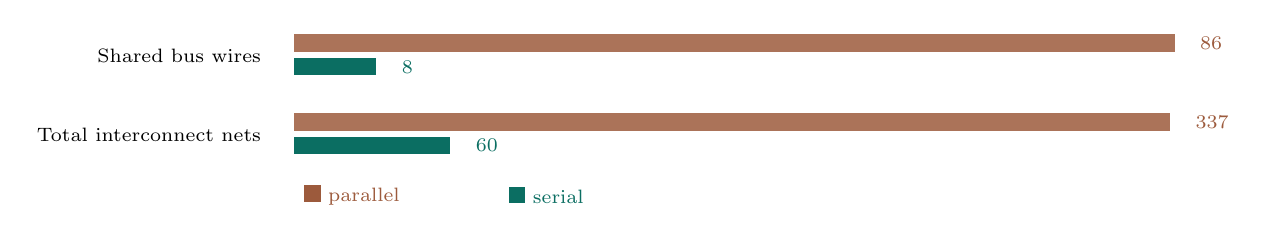
\begin{tikzpicture}[font=\scriptsize,x=1mm,y=1cm]
  \foreach \lbl/\p/\s/\y/\k in {%
    {Shared bus wires}/86/8/1.0/1.30,
    {Total interconnect nets}/337/60/0.0/0.33}{
    \node[anchor=east,font=\scriptsize] at (-3,\y+0.27) {\lbl};
    \fill[legacy!85] (0,\y+0.32) rectangle (\p*\k,\y+0.54);
    \fill[signal]    (0,\y+0.02) rectangle (\s*\k,\y+0.24);
    \node[anchor=west,font=\scriptsize,color=legacy] at (\p*\k+2,\y+0.43) {\p};
    \node[anchor=west,font=\scriptsize,color=signal] at (\s*\k+2,\y+0.13) {\s};}
  \node[anchor=west,color=legacy,font=\scriptsize] at (0,-0.5)
    {\textcolor{legacy}{\rule{6pt}{6pt}}\ parallel};
  \node[anchor=west,color=signal,font=\scriptsize] at (26,-0.5)
    {\textcolor{signal}{\rule{6pt}{6pt}}\ serial};
\end{tikzpicture}
\caption{Wire count. Bars are scaled independently per row.}
\end{figure}

\begin{table}[htb]
\centering\small
\caption{Serial bus net count.}
\begin{tabular}{@{}lrrr@{}}
\toprule
\textbf{Segment} & \textbf{Per unit} & \textbf{Units} & \textbf{Nets}\\
\midrule
Master $\rightarrow$ forward mux (private) & 4  & 2 & 8\\
Shared bus                                 & 8  & 1 & 8\\
Slave $\rightarrow$ return mux (private)   & 4  & 4 & 16\\
Arbitration and select                     & 11 & 1 & 11\\
Decode path inside \sig{system\_bus}       & 17 & 1 & 17\\
\midrule
\multicolumn{3}{@{}l}{\textbf{Total}} & \textbf{60}\\
\bottomrule
\end{tabular}
\end{table}

\subsection{Latency}

All figures measured in simulation, from command acceptance to completion.

\begin{table}[htb]
\centering\small
\caption{Transaction cost. The nine-clock gap between a write and a read is
exactly the read data phase.}
\begin{tabular}{@{}lrr@{}}
\toprule
& \textcolor{legacy}{\textbf{Parallel}} & \textcolor{signal}{\textbf{Serial}}\\
\midrule
Write                                  & 5\,clk  & 21\,clk\\
Read                                   & 5\,clk  & 30\,clk\\
Read, contended (winner / loser)       & 5 / 9   & 30 / 59\\
Split read (\sig{SPLIT\_LATENCY}${=}6$) & 16\,clk & 79\,clk\\
\bottomrule
\end{tabular}
\end{table}

Sixteen of a read's thirty clocks are the address going out one bit at a
time. That is the dominant term, and it is the price of a one-wire address.

\subsection{Implementation}

\begin{table}[htb]
\centering\small
\caption{Quartus Prime Lite 24.1std, \sig{EP4CE115F29C7}, full
map / fit / sta / asm flow.}
\begin{tabular}{@{}lrr@{}}
\toprule
& \textcolor{legacy}{\textbf{Parallel}} & \textcolor{signal}{\textbf{Serial}}\\
\midrule
Errors               & 0 & 0\\
Inferred latches     & 0 & \textbf{0}\\
Combinational loops  & 0 & \textbf{0}\\
Logic elements       & 721 & \textbf{688}\\
Registers            & 544 & \textbf{513}\\
Memory bits (all M9K)& 327{,}680 & 81{,}920\\
$F_{\max}$ (slow, 1200\,mV, 85\,$^\circ$C) & 117.7\,MHz & \textbf{141.8\,MHz}\\
\bottomrule
\end{tabular}
\end{table}

The serial bus is \emph{smaller and faster} than the parallel bus it
replaced, which was not the expected outcome. Two effects explain it: the
32-bit forward and return multiplexers cost more logic than the shift
registers that replaced them, and the widest combinational path on the bus
--- the return multiplexer --- is now one bit wide instead of thirty-two.
Timing closes with a $2.8\times$ margin on the 50\,MHz requirement.

%==========================================================================
\section{Limitations and further work}
\label{sec:limits}

\begin{description}[leftmargin=1.4em,style=nextline,font=\bfseries]
\item[Fixed priority can starve the low-priority master.]
With master~0 requesting continuously, master~1 never runs. The bus lock
bounds the wait to one transfer, but priority is priority. Round-robin or a
weighted scheme would fix it; the arbiter's structure supports either without
touching anything else.

\item[The address frame dominates latency.]
Sixteen of thirty clocks carry an address that is usually close to the
previous one. Two obvious improvements: pipeline the next frame against the
current data phase, or send a short frame when the upper address bits are
unchanged. Both were out of scope; both are worth more than any other
optimisation available.

\item[One split outstanding.]
A second split-capable slave, or a second outstanding split on slave~0, would
need per-master deferred state and one wake-up per entry.

\item[Board demo throttling, not clock division.]
The specification asked for a PLL or clock divider to slow the demo down. A
divided clock is a derived clock and would violate the project's own
one-domain, no-gated-clock rule, so the bus runs at 50\,MHz and only the
scenario sequencer is throttled by a slow clock-enable tick. Same visible
effect, one clock domain, fully timing-analysable.

\item[Memory contents are undefined at power-up.]
The arrays are deliberately unreset --- an asynchronous reset on a 4096-word
array stops M9K inference and builds the memory from flip-flops instead ---
so every test writes a location before reading it.
\end{description}

\paragraph{Phase 2 readiness.} The remote bridge joins as a third bus
requester. Three things were arranged in advance: the arbiter is
parameterised on \sig{N\_MASTERS} and already exercises splits on both a
high- and a low-priority master; the split mechanism is written once and is
enabled by a single parameter on any slave; and \sig{addr[15]}${=}1$ is
reserved and unmapped, with an exhaustive 64K decoder sweep that fails if
anything is ever mapped there.

%==========================================================================
\section{Conclusion}

The bus does what was asked: two masters, three slaves, priority arbitration
with a bus lock, address decoding with a guaranteed responder, and split
transactions --- with the address and the data each carried on a single
shared wire.

The engineering judgement that mattered most was not any of the protocol
mechanisms; it was \textbf{right-aligning the write data inside the address
frame} (\S\ref{sec:frame}). That one choice turns every receiver on the bus
into a plain shift register holding ``the last $W$ bits I saw'', removes bit
counters from four different modules, and leaves exactly one frame timer in
the entire system. It cost eight cycles of padding on a write --- cycles the
address phase was going to spend anyway --- and bought a bus with no
distributed timing state at all.

The second was recognising that serialisation does not merely slow a bus
down: it changes which mechanisms are worth having. A split transaction that
saved five clocks on the parallel bus saves thirty on this one, and a
mechanism that looked like a specification box to tick became the part of the
design doing the most work.

%==========================================================================
\appendix
\section{Module inventory}

\begin{table}[htb]
\centering\small
\begin{tabularx}{\textwidth}{@{}llX@{}}
\toprule
\textbf{Module} & \textbf{Role} & \textbf{Notes}\\
\midrule
\sig{system\_bus}    & the bus     & arbiter, decoder, mux, address
                                     deserialiser, default responder\\
\sig{arbiter}        & scheduling  & fixed priority, bus lock, split mask;
                                     parameterised on \sig{N\_MASTERS}\\
\sig{addr\_decoder}  & decode      & purely combinational, one-hot + default\\
\sig{bus\_mux}       & data path   & who drives the two shared wires;
                                     latched return select\\
\sig{shift\_ser}     & primitive   & parallel in, serial out; pads with zeros\\
\sig{shift\_deser}   & primitive   & serial in, parallel out; holds the last
                                     $W$ bits\\
\sig{default\_slave} & bus service & answers \sig{ERROR} for unmapped
                                     addresses\\
\sig{master}         & endpoint    & serialises, replays after \sig{SPLIT}\\
\sig{slave}          & endpoint    & memory; \sig{SPLIT\_CAPABLE} adds split
                                     state\\
\sig{bus\_top}       & integration & masters + bus + slaves, no logic\\
\sig{de2\_top}       & board       & clocking, buttons, switches, displays\\
\bottomrule
\end{tabularx}
\end{table}

\section{Address map}

\begin{table}[htb]
\centering\small
\begin{tabular}{@{}llll@{}}
\toprule
\textbf{Range} & \textbf{Responder} & \textbf{Size} & \textbf{Decode}\\
\midrule
\sig{0x0000}--\sig{0x0FFF} & slave 0 & 4\,KB & \sig{addr[15:12]==4'h0}\\
\sig{0x1000}--\sig{0x1FFF} & slave 1 & 4\,KB & \sig{addr[15:12]==4'h1}\\
\sig{0x2000}--\sig{0x27FF} & slave 2 & 2\,KB & \sig{addr[15:11]==5'b00100}\\
\sig{0x2800}--\sig{0x2FFF} & default & ---   & decode hole\\
\sig{0x3000}--\sig{0x7FFF} & default & ---   & unmapped\\
\sig{0x8000}--\sig{0xFFFF} & default & ---   & \textbf{reserved}, phase-2
                                               remote window\\
\bottomrule
\end{tabular}
\end{table}

Slave 0 is the split-capable one. Every unmapped range answers \sig{ERROR} on
the normal one-cycle schedule, so no address in the 64K space can stall the
bus.

\end{document}
